\documentclass[11pt]{article}
\usepackage{amsmath,amsthm,amssymb}
\usepackage{pgfplots}
	\usetikzlibrary{
		calc,
		patterns,
		positioning
	}
	\pgfplotsset{
		compat=1.16,
		samples=200,
		clip=false,
		my axis style/.style={
			axis x line=middle,
			axis y line=middle,
			legend pos=outer north east,
			axis line style={
				->,
			},
			legend style={
				font=\footnotesize
			},
			label style={
				font=\footnotesize
			},
			tick label style={
				font=\footnotesize
			},
			xlabel style={
				at={
					(ticklabel* cs:1)
				},
				anchor=west,
				font=\footnotesize,
			},
			ylabel style={
				at={
					(ticklabel* cs:1)
				},
				anchor=west,
				font=\footnotesize,
			},
			xlabel=$t$,
			ylabel=$u(t)$
		},
	}
	\tikzset{
		>=stealth
	}
 \usepackage{float}
\usepackage{caption}
	\captionsetup{
		format=plain,
		labelfont=bf,
		font=small,
		justification=centering
	}
 \newcommand{\E}{\mathrm{e}}
\usepackage[utf8]{inputenc}	% Para caracteres en español
\usepackage{amsmath,amsthm,amsfonts,amssymb,amscd}
\usepackage{multirow,booktabs}
\usepackage[table]{xcolor}
\usepackage{fullpage}
\usepackage{lastpage}
\usepackage{enumitem}
\usepackage{fancyhdr}
\usepackage{mathrsfs}
\usepackage{wrapfig}
\usepackage{setspace}
\usepackage{calc}
\usepackage{multicol}
\usepackage{cancel}
\usepackage[retainorgcmds]{IEEEtrantools}
\usepackage[margin=3cm]{geometry}
\usepackage{amsmath}
\newlength{\tabcont}
\setlength{\parindent}{0.0in}
\setlength{\parskip}{0.05in}
\usepackage{empheq}
\usepackage{framed}
\usepackage[most]{tcolorbox}
\usepackage{xcolor}
\colorlet{shadecolor}{gray!15}
\parindent 0in
\parskip 12pt
\geometry{margin=1in, headsep=0.25in}
\theoremstyle{definition}
\newtheorem{defn}{Definition}
\newtheorem{class}{Classification}
\newtheorem{ex}{Example}
\newtheorem{note}{Note}
\newtheorem*{note*}{Note}
\newtheorem{thm}{Theorem}
%\theoremstyle{definition}
\begin{document}
\setcounter{section}{0}
\title{Chapter 9 Review Notes}

\thispagestyle{empty}

\begin{center}
{\LARGE \bf MAT292: Ordinary Differential Equations (Weeks 1-2)}\\
{\large Rizzmaster9000}\\
Fall 2023
\end{center}
\section{Introduction}
\subsection{Mathematical Models and Solutions}
\textsc{Differential Equations} are equations relating a function and its derivatives. They are useful for modelling the behaviour of the natural world.
\colorlet{shadecolor}{blue!15}\begin{shaded}
\textbf{Newton's Law of Cooling}\\
Let $u(t)$ be an object's temperature at time $t$, and let $T$ be the temperature of the object's surroundings. Then $u'(t) = \frac{du}{dt}$ is the rate of change of the object's temperature. Newton found that $u'$ is proportional to $-(u(t) - T)$ via a positive coefficient $k$, thus yielding the differential equation \begin{equation}
    \frac{du}{dt} = -k(u(t) - T)
\end{equation} as a model for the situation.
\end{shaded}Assuming from now on that $T$ is a constant value $T_0$, we introduce the following terminology to describe the quantities in (1):\\\\\textcolor{red}{$t$ is an \textsc{independent} variable,\\ $u(t)$ is a \textsc{dependent} variable since it depends on $t$, and\\ $k$, $T_0$ are \textsc{parameters} in the model.}\\\\ This equation is an \textsc{Ordinary Differential Equation (ODE)} since it only has one independent variable. When it comes to such equations, we have two main questions:\\\\
"Does a function $u(t)$ exist such that the equation is true for all $t$?"\\
"If the equation has a solution, how can we find it?"\\\\
Answering these questions is the main purpose of this course.\\\\
\textsc{Solutions} to differential equations are functions which satisfy said equations. One solution of (1) is $u(t) = T_0$, since both sides reduce to 0. This type of solution is called an \textsc{Equilibrium Solution}.
\\\\If we assume that $u(t) \neq T_0$, other solutions can be discovered by rewriting (1) in the form
\begin{equation}
\frac{\frac{du}{dt}}{u(t) - T_0} = -k
\end{equation}
By the chain rule, the left side of (2) is the derivative of $\ln{|u(t) - T_0|}$ with respect to $t$, so
\begin{equation}
\frac{d}{dt}\ln{|u(t) - T_0|} = -k
\end{equation}
Now, integrating both sides with respect to $t$ and exponentiating both sides,
\begin{equation}
\ln{|u(t) - T_0|} = -kt + C
\end{equation}
\begin{equation}
|u(t) - T_0| = e^{-kt + C} = e^{-kt}e^C
\end{equation}
Removing the absolute value sign and isolating $u(t)$, we find that the solution to (1) is
\begin{equation}
u(t) = ce^{-kt} + T_0
\end{equation}
where $c = \pm e^C$. Note that if we set $c = 0$, the equilibrium solution $u = T_0$ is also contained in (6). (6) contains all possible solutions to (1) and is called the \textsc{General Solution} of the equation.\\\\
\textsc{Integral Curves} are the geometric representations of general solutions of ODEs. They consist of an infinite family of curves satisfying (6), but with different values of $c$ for each curve. For example, the family of curves for the equation \begin{equation}u(t) = 30 + ce^{-1.5t}\end{equation} looks like this for selected values of $c$:
\begin{figure}[h]
	\centering
	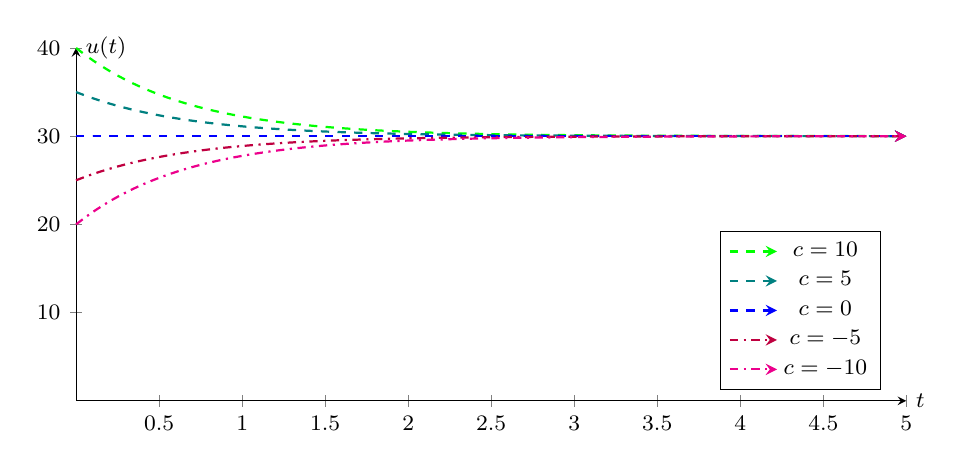
\begin{tikzpicture}
	\begin{axis}[
		my axis style,
		width=\textwidth,
		height=.5\textwidth,
        ymax = 40,
        ymin = 0,
		legend entries={
			$c = 10$,
			$c = 5$,
			$c = 0$,
                $c = -5$,
                $c = -10$,
		},
		legend pos=south east
	]

        \addplot[
		domain=0:5,
		thick,
		green,
		dashed,
		->
	]
	{30 + 10*exp(-1.5*x)};

	\addplot[
		domain=0:5,
		thick,
		teal,
		dashed,
		->
	]
	{30 + 5*exp(-1.5*x)};

        \addplot[
		domain=0:5,
		thick,
        blue,
        dashed,
		->
	]
	{30};

	\addplot[
		domain=0:5,
		thick,
		purple,
		dashdotted,
		->
	]
	{30 - 5*exp(-1.5*x)};

        \addplot[
		domain=0:5,
		thick,
		magenta,
		dashdotted,
		->
	]
	{30 - 10*exp(-1.5*x)};

	%\fill[
		%black
	%]
	%(1,.36788) circle (2pt) node[above right] {\footnotesize %$(1, 1/\E)$};

	\end{axis}
	\end{tikzpicture}
	\caption{Integral curves for the equation $u(t) = 30 + ce^{-1.5t}$}
	\label{fig:my-awesome-graph}
\end{figure}
\\Often, we may wish to focus on a single curve from the infinite possibilities in the general solution. To do so, we will need to specify \textsc{Initial Conditions}. For example, for (7) we might be interested in the solution when the temperature is equal to 70 at time $t = 0$. Plugging these values into the equation, we get \begin{equation}70 = 30 + c\end{equation}so $c = 40$ and the solution for the given initial conditions turns out to be \begin{equation}u(t) = 30 + 40e^{-1.5t}\end{equation}
\newpage
\subsection{Definitions, Classifications, and Terminology}
To summarize what we have learned thus far, here are important definitions from the preceding section, as well as some mathematical terminology and the various ways in which differential equations are classified.
\colorlet{shadecolor}{gray!15}\begin{shaded}
\begin{defn}
\textbf{Order} - The order of a differential equation is the order of the highest derivative, either ordinary or partial, that appears in said equation.
\end{defn}
\end{shaded}
\begin{ex} The equation
\begin{equation}
f(t) = ay'''(t) + by''(t)
\end{equation}
is a third order ODE.
\end{ex}
\begin{note*}
    The notation \begin{equation}
        F[t, y, y', ..., y^{(n)}] = 0, \text{ or equivalently, }y^{(n)} = f(t, y, y', ..., y^{(n-1)})
    \end{equation} can be used to represent the equation of an $n$th order ODE.
\end{note*}
\begin{shaded}
\begin{defn}
\textbf{Linear} - An $n$th order ODE is \textsc{Linear} if it can be expressed in the form \begin{equation}a_0(t)u(t) + a_1(t)u'(t) + ... + a_n(t)u^{(n)}(t) = g(t)\end{equation} If $g(t) = 0$ for all $t$, then (0) is \textsc{Homogeneous}; if not, (0) is \textsc{Nonhomogeneous}.
\end{defn}
\end{shaded}
\begin{ex}
    $t\sin{(t^3)}u(t) + 56u'''(t) + t^4 = 0$ is linear because, if we move $t^4$ to the other side of the equation, we get
    \begin{equation}t\sin{(t^3)}u(t) + 56u'''(t) = -t^4\end{equation} which is of the form shown in (12). Since the right hand side is not the zero function, (x) is nonhomogeneous.
\end{ex}
\begin{ex}
    $tu(t) + 5\sqrt{u'(t)} + 10\sin{(u(t))} = 0$ is nonlinear because it is impossible to manipulate the second and third terms such that this equation takes the form in (12).
\end{ex}
\begin{shaded}
\begin{defn}
\textbf{Autonomous} - An ODE is \textsc{Autonomous} if it can be expressed in the form \begin{equation}\frac{dy}{dt} = f(y)\end{equation}In other words, an ODE is autonomous if it does not explicitly depend on the independent variable.
\end{defn}
\end{shaded}
\begin{ex}
   $\frac{dy}{dt} = \sin{(y)} + y^3\ln{(y)} + e^y$ is autonomous.
\end{ex}
\begin{ex}
   $\frac{dy}{dt} = \sin{(ty)}$ is not autonomous, since the independent variable $t$ appears on the right hand side of the equation.
\end{ex}
\begin{class}
\textbf{System of Differential Equations} - A system of differential equations occurs when two or more independent variables interact with one another.
\end{class}
\colorlet{shadecolor}{blue!15}\begin{shaded}
    \textbf{Lotka-Volterra Equations}\\
    The Lotka-Volterra (a.k.a. predator-prey) equations are of the form \begin{equation}
        \frac{dx}{dt} = ax - \beta xy,\,\,\,\,
        \frac{dy}{dt} = -cx + \gamma xy
    \end{equation} where $x(t)$, $y(t)$ represent the respective populations of the prey and predator species. This system assumes that the prey will only die when eaten, and that predators either naturally die or relocate. The behaviour of the system is periodic, with $y(t)$ lagging behind $x(t)$.
\end{shaded}
\colorlet{shadecolor}{gray!15}\begin{shaded}
\begin{defn}
\textbf{Solution} - A \textsc{solution} of an ODE on the interval $a \leq t\leq b$ is a function $u(t)$ such that $u'(t), u''(t), ..., u^{(n)}(t)$ exist and satisfy \begin{equation}
u^{(n)}(t) = f(t, u(t), u'(t), ..., u^{(n - 1)}(t))
\end{equation}
\end{defn}
\end{shaded}
\begin{ex}
    $u_1(t) = \cos{t}$ and $u_2(t) = \sin{t}$ are solutions of the differential equation \begin{equation}
        u''(t) + u(t) = 0
    \end{equation} for all $t$ because, plugging $u_1(t)$ and $u_2(t)$ into (0), we get \begin{equation}
        -\cos{t} + \cos{t} = 0\text{ and }-\sin{t} + \sin{t} = 0
    \end{equation}
\end{ex}
\begin{shaded}
    \begin{defn}
    \textbf{Initial Value Problem} - An \textsc{Initial Value Problem (IVP)} for an $n$th order ODE on an interval $I$ consists of (12) together with $n$ initial conditions \begin{equation}
        y(t_0) = y_0,\,\,\, y'(t_0) = y_1,\,\,\, ...,\,\,\, y^{(n-1)}(t_0) = y_{n - 1}
    \end{equation} prescribed at a point $t_0 \in I$, where $y_0,\, y_1,\,...,\,y_{n-1}$ are constants.
\end{defn}
\end{shaded}
\begin{ex}
$v(t) = 2\cos{t} - 3\sin{t}$ is a solution for all $t$ to the IVP consisting of (18) and initial conditions $u(0) = 2$, $u'(0) = -3$. Plugging $v(t)$ into (18), we find that \begin{equation}
        v''(t) + v(t) = -2\cos{t} + 3\sin{t} + 2\cos{t} - 3\sin{t} = 0
    \end{equation} which means that $v(t)$ is a solution to (18) for all $t$. Checking the initial conditions, we find that \begin{equation}
        v(0) = 2\cos{0} - 3\sin{0} = 2,\,\,\,\,v'(0) = -2\sin{0} - 3\cos{0} = -3
    \end{equation} which means the initial conditions are satisfied as well; hence, $v(t)$ is a solution to the IVP.
\end{ex}
\newpage
\section{First Order Differential Equations}
\subsection{Separable Equations}
A general first order differential equation is of the form \begin{equation}
    \frac{dy}{dx} = f(x,y)
\end{equation}
In this section, we consider cases where the right hand side of (22) takes on a special form.
\begin{shaded}
\begin{defn}
\textbf{Separable} - A first order equation is \textsc{Separable} if it can be expressed in the form \begin{equation}
    \frac{dy}{dx} = f(x,y) = p(x)g(y)
\end{equation} In other words, a separable equation can be expressed as the product of a function $p(x)$ depending exclusively on $x$ and a function $g(y)$ depending exclusively on $y$.
\end{defn}
\end{shaded}
\begin{note*}
    We can also show an equation is separable by expressing it in the form \begin{equation}
    M(x) + N(y)\,\frac{dy}{dx} = 0 = M(x)\,dx + N(y)\,dy
\end{equation} where $M(x),\, N(y)$ can be different from $p(x),\, g(y)$.
\end{note*}
\begin{ex}
    The first order ODE \begin{equation}
        \frac{dy}{dx} = \frac{x^2}{1 - y^2}
    \end{equation} is separable since we can choose $p(x) = x^2$, $g(y) = \frac{1}{1 - y^2}$.
\end{ex} The general method for solving a separable equation is to rearrange terms so that one side is exclusively in terms of $y$ and the other side is exclusively in terms of $x$, and then integrate both sides and rearrange as necessary. \begin{ex}
    To solve \begin{equation}
        \frac{dy}{dx} = \frac{x^2}{y^2}
    \end{equation}we rearrange and integrate as follows: \begin{equation}
        \int y^2\,dy = \int x^2\,dx
    \end{equation}
    \begin{equation}
        \frac{y^3}{3} = \frac{x^3}{3} + c
    \end{equation}
    \begin{equation}
        y = \sqrt[3]{x^3 + k}
    \end{equation} where $k = 3c$. (0) is the \textsc{explicit solution} of the differential equation.
\end{ex}
\begin{ex}
    To solve the IVP \begin{equation}
        \frac{dr}{d\theta} = \frac{r^2}{\theta},\,\,\, r(1) = 2
    \end{equation}we rearrange and integrate as follows: \begin{equation}
        \int\frac{1}{r^2}\,dr = \int\frac{1}{\theta}\,d\theta
    \end{equation}
    \begin{equation}
        \frac{-1}{r} = \ln{|\theta|} + c
    \end{equation}
    \begin{equation}
        r = \frac{-1}{\ln{|\theta|} + c}
    \end{equation}
\end{ex}
Plugging in the initial condition, we have $2 = \frac{-1}{\ln{|1|} + c}$, so $c = \frac{-1}{2}$ and the explicit solution of the differential equation turns out to be \begin{equation}
    r = \frac{-1}{\ln{|\theta|} - \frac{1}{2}}
\end{equation} Now we need to find the \textcolor{red}{\textsc{interval of validity}} for the solution, which requires\\\\ \textcolor{red}{$i)$ that the interval contains the value of the independent variable specified in the IVP ($\theta = 1$ in this case), and\\ $ii)$ that the interval is continuous with no breaks or holes.}\\\\ Noticing that $r$ is undefined at the values $\theta = 0, \,\pm{e^{\frac{1}{2}}}$, we obtain 4 possible intervals of validity: \begin{equation}
    -\infty < \theta < -\sqrt{e},\,\,\, -\sqrt{e} < \theta < 0,\,\,\, 0 < \theta < \sqrt{e},\,\,\, \sqrt{e} < \theta < \infty
\end{equation} Since the IVP specified that $\theta = 1$, we see that the explicit solution we have obtained is only valid on the interval $0 < \theta < \sqrt{e}$.
\begin{ex}
    To solve the IVP \begin{equation}
        \frac{dy}{dt} = e^{y - t}\sec{(y)}(1 + t^2),\,\,\, y(0) = 0
    \end{equation} we rearrange and integrate as follows:\begin{equation}
        \int \frac{1}{e^y}\cos(y)\,dy = \int e^{-t}(1 + t^2)\,dt
    \end{equation}
    \begin{equation}
        \frac{1}{2e^y}(\sin{y} - \cos{y}) = -e^{-t}(t^2 + 2t + 3) + c
    \end{equation} Plugging in the initial condition, we have $\frac{-1}{2} = -3 + c$, so $c = \frac{5}{2}$ and the \textsc{implicit solution} of the differential equation turns out to be \begin{equation}
        \frac{1}{2e^y}(\sin{y} - \cos{y}) = -e^{-t}(t^2 + 2t + 3) + \frac{5}{2}
    \end{equation}
\end{ex} It is impossible to convert this solution into an explicit form, so we leave it as is.
\begin{note*}
    Since finding intervals of validity for implicit solutions can typically be very difficult without a graph, we will avoid doing so throughout this document.
\end{note*}
\subsection{Linear Equations: Method of Integrating Factors}
While it is impossible to find an analytic solution for every first order ODE, we can use a special method to solve every $\color{red}{\textsc{linear first order ODE}}$, i.e., every ODE which can be expressed as \begin{equation}
    \color{red}{\frac{dy}{dt} + p(t)y = g(t)}
\end{equation}
To do so, we introduce an unknown function $o(t)$, and assume that $o(t)$ is positive and $o'(t) = o(t)p(t)$, i.e., \begin{equation}
    \frac{do}{dt} = o(t)p(t)
\end{equation} \begin{equation}
    \frac{1}{o(t)}\frac{do}{dt} = g(t)
\end{equation} Integrating both sides, we have \begin{equation}
    \ln{|o(t)|} = \int g(t)\,dt + k
\end{equation} where $k$ is an arbitrary constant. If we choose $k = 0$, then by exponentiating both sides we obtain the value of the $\color{red}{\textsc{integrating factor}}$ $o(t)$: \begin{equation}
    \color{red}{o(t) = e^{\int p(t)\,dt}}
\end{equation}Now we multiply both sides of (41) by the integrating factor:\begin{equation}
    o(t)\frac{dy}{dt} + o(t)p(t)y = o(t)g(t)
\end{equation} and the left hand side is just the derivative of $o(t)y$ by the product rule, so we have \begin{equation}
    o(t)y = \int o(t)g(t)\,dt + c
\end{equation} and the general solution to (41) is \begin{equation}
    y = \frac{1}{o(t)}\Bigg[\int o(t)g(t)\,dt + c\Bigg]
\end{equation}To summarize the process:
\colorlet{shadecolor}{green!15}\begin{shaded}
\textbf{Method of Integrating Factors for Linear First Order ODES}\\
I. Put the equation in the form shown in (41).\\
II. Calculate the integrating factor $o(t) = e^{\int p(t)\,dt}$.\\
III. Multiply (41) by $o(t)$ and put it in the form $[o(t)y]' = o(t)g(t)$.\\
IV. Integrate both sides and separate for $y$ so that you get the equation in (48).\end{shaded}As mentioned, this method works for any linear first order ODE. The important results yielded from it are the integrating factor $o(t)$ and the general solution in the form shown in (48).\begin{note*}
    It may be useful to memorize the formula in (45); however, the formula in (48) should not be memorized until you are comfortable solving problems by following the entire process for the method of integrating factors. This is because you want to be able to understand the procedure instead of blindly applying it and risking errors.
\end{note*}\begin{ex}
    To solve the linear first order ODE \begin{equation}
        \frac{dy}{dx} + 3x^2y = 6x^2
    \end{equation} we take the integrating factor as\begin{equation}
        o(t) = e^{\int 3x^2\,dx} = e^{x^3}
    \end{equation}Then \begin{equation}
        e^{x^3}\frac{dy}{dx} + e^{x^3}3x^2y = e^{x^3}6x^2
    \end{equation}which can be equivalently expressed using the product rule as \begin{equation}
        [e^{x^3}y]' = e^{x^3}6x^2
    \end{equation}
    Integrating both sides and separating for $y$, we obtain the general solution \begin{equation}
    y = \frac{1}{e^{x^3}}\Bigg[\int e^{x^3}6x^2\,dx + c\Bigg] = 2 + \frac{c}{e^{x^3}}
\end{equation}
\end{ex}\begin{ex}
    To solve the IVP \begin{equation}
        ty' + 2y = 4t^2,\,\,\, y(1) = 2
    \end{equation}we begin by dividing the equation by $t$ to obtain the form in (41):\begin{equation}
        y' + \frac{2}{t}y = 4t
    \end{equation}Then the integrating factor is \begin{equation}
        o(t) = e^{\int\frac{2}{t}\,dt} = e^{2\ln{|t|}} = t^2
    \end{equation}Multiplying (54) by (55), we have \begin{equation}
        t^2y' + t^2\frac{2}{t}y = t^24t
    \end{equation} and taking advantage of the product rule, \begin{equation}
        [t^2y]' = 4t^3
    \end{equation}Integrating both sides and separating for $y$, we obtain the general solution \begin{equation}
        y = \frac{1}{t^2}\Bigg[\int 4t^3\,dt + c\Bigg] = t^2 + \frac{c}{t^2}
    \end{equation} Plugging in $y(1)$ = 2, we have \begin{equation}
        y = t^2 + \frac{2}{t^2}
    \end{equation} as the explicit solution. If $c \neq 0$, $y$ is undefined when $t = 0$ and continuous everywhere else, so we have two possible intervals of validity: \begin{equation}
        t < 0,\,\,\, t > 0
    \end{equation}Since it was given in the IVP that $t = 1$, the interval of validity for (60) is $t > 0$.
\end{ex}
\subsection{Modelling with First Order Equations}
In this section, we provide examples of real-world scenarios which can be modelled via first order ODEs.
\begin{ex}
    An object of constant mass $m$ is launched away with initial velocity $v_0$ from the Earth in a direction perpendicular to its surface. Obtain an equation for its velocity $v$, the initial velocity required to propel it to a maximum altitude above the Earth, and the least initial velocity (i.e. escape velocity) which will allow the object to escape the Earth's gravitational pull.
\end{ex}
Let $x$ be the height of the object relative to the earth's surface. The gravitational force acting on the object $F(x)$ is inversely proportional to the square of the object's distance from the center of the earth; hence, we start with the equation \begin{equation}
    F(x) = \frac{-k}{(x + R)^2}
\end{equation} where $k$ is a constant, $R$ is the earth's radius, and the minus sign signifies that $F(x)$ is directed in the negative $x$ direction. Since $w(0) = -mg$, $k = mgR^2$, and since $F(x) = m\frac{dv}{dt}$, we have \begin{equation}
    m\frac{dv}{dt} = \frac{-mgR^2}{(x + R)^2}
\end{equation} There are too many variables in this equation, since it depends on $x$, $t$, and $v$; however, we can fix this by taking $x$ as the independent variable instead of $t$. Then we need to use the chain rule to express $\frac{dv}{dt}$ in terms of $x$, before plugging the result back into (63): \begin{equation}
    \frac{dv}{dt} = \frac{dv}{dx}\frac{dx}{dt} = v\frac{dv}{dx}
\end{equation}
\begin{equation}
    v\frac{dv}{dx} = \frac{-gR^2}{(x + R)^2}
\end{equation} which is a separable differential equation and hence solvable using methods we have already learned: \begin{equation}
    \frac{v^2}{2} = \frac{gR^2}{x + R} + c
\end{equation} At the initial condition $x = 0$, we were given that $v = v_0$, so we can simply replace $v$ with $v_0$ to get $c = \frac{v_0^2}{2} - gR$, which gives us the equation of $v$:\begin{equation}
    v = \pm{\sqrt{v_0^2 - 2gR + \frac{2gR^2}{x + R}}}
\end{equation} The maximum altitude occurs when $v = 0$, so plugging this value in and separating for $v_0$ we get:\begin{equation}
    x = \frac{v_0^2R}{2gR - v_0^2},\,\,\, v_0 = \sqrt{2gR\frac{x}{x + R}}
\end{equation} The escape velocity can be obtained by letting $x \rightarrow{\infty}$:\begin{equation}
    v_0 = \sqrt{2gR}
\end{equation}\newpage
\begin{ex}
    A pond contains 10 million gallons of fresh water. Water containing diarrhea enters the pond at a rate of 5 million gallons per year, and the mixture in the pond overflows out of the pond at the same rate. The concentration of diarrhea in the incoming water is given by the function $P(t) = 2 + \sin{2t}$ g/gal, where $t$ is measured in years. Obtain a function which determines the amount of diarrhea in the pond at any time.
\end{ex} Denote the mass of diarrhea in grams in the pond as $D(t)$. Then we have the equation \begin{equation}
    \frac{dD}{dt} = \text{rate in} - \text{rate out}
\end{equation} The rate at which the diarrhea flows into the pond is given by \begin{equation}
    (5 * 10^6)\text{gal/year $*$ }(2 + \sin{2t})\text{g/gal}
\end{equation} Since the amount of water in the pond remains constant at $10^7$ gallons, the concentration of diarrhea in the pond is $\frac{D(t)}{10^7}$ g/gal. Thus the rate at which the diarrhea flows out of the pond is given by  \begin{equation}
    (5 * 10^6)\text{gal/year $*$ }\left(\frac{D(t)}{10^7}\right)\text{g/gal} = \left(\frac{D(t)}{2}\right)\text{g/year}
\end{equation} We then have the differential equation \begin{equation}
    \frac{dD}{dt} = (5 * 10^6)(2 + 2\sin{2t}) - \frac{D(t)}{2}
\end{equation}where each term has the units of g/year, as a model for our problem. For convenience, we introduce a new function $d(t) = \frac{D(t)}{10^6}$ which gets rid of the large coefficients in (73). In physical terms, $d(t)$ measures the mass of diarrhea in megagrams in the pond. Substituting $d(t)$ for $D(t)$ and rearranging terms, we obtain the equation \begin{equation}
    \frac{dd}{dt} + \frac{d}{2} = 10 + 5\sin{2t}
\end{equation}Being a linear first order equation, the integrating factor is $e^{\frac{t}{2}}$, so applying the method of integrating factors we get \begin{equation}
    d(t) = 20 - \frac{40}{17}\cos{2t} + \frac{10}{17}\sin{2t} + ce^{\frac{-t}{2}}
\end{equation} and since the initial condition is $d(0) = 0$ due to no diarrhea being in the pond at the start,\begin{equation}
    d(t) = 20 - \frac{40}{17}\cos{2t} + \frac{10}{17}\sin{2t} - \frac{300}{17}e^{\frac{-t}{2}}
\end{equation}is the explicit solution to the IVP.\begin{figure}[h]
	\centering
	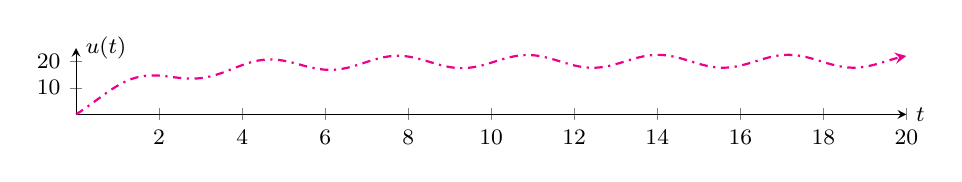
\begin{tikzpicture}
	\begin{axis}[
		my axis style,
		width=\textwidth,
		height=.2\textwidth,
        ymax=25,
	]
        \addplot[
		domain=0:20,
		thick,
		magenta,
		dashdotted,
		->
	]
	{20 - (40/17)*cos(deg(2*x)) + (10/17)*sin(deg(2*x)) - (300/17)*exp(-0.5*x)};

	%\fill[
		%black
	%]
	%(1,.36788) circle (2pt) node[above right] {\footnotesize %$(1, 1/\E)$};

	\end{axis}
	\end{tikzpicture}
	\caption{Graph of the explicit solution $d(t) = 20 - \frac{40}{17}\cos{2t} + \frac{10}{17}\sin{2t} - \frac{300}{17}e^{\frac{-t}{2}}$}
	\label{fig:my-awesome-graph}
\end{figure}
\subsection{Differences between Linear and Nonlinear Equations}
Thus far, we have only considered IVPs with one solution. However, this is not the case for all IVPs; conditions for the existence and uniqueness of solutions to a linear first order IVP are given by the following theorem.\colorlet{shadecolor}{gray!15} \begin{shaded}\begin{thm}
    \textbf{Existence and Uniqueness (Linear Only)} - If $p,\,g$ are continuous functions on an open interval $I = (\alpha, \beta)$ containing the point $t = t_0$, and $y_0$ is an arbitrary prescribed initial value, then there exists a unique function $y$ which is a solution to the linear first order IVP \begin{equation}
        y' + p(t)y = g(t),\,\,\,y(t_0) = y_0
    \end{equation} for all $t \in I$.
\end{thm}\end{shaded}
For nonlinear first order IVPs, more rigorous conditions are required to guarantee the existence and uniqueness of solutions.
\begin{shaded}\begin{thm}
    \textbf{Existence and Uniqueness (Linear + Nonlinear)} - If $p$ is a continuous function on an open rectangle $R = \{(x,y)\,\,|\,\,\alpha < x < \beta,\, \gamma < y < \delta\}$ containing a point $(x_0, y_0)$, then there exists a unique function $y = g(x)$ which is a solution to the IVP \begin{equation}
        y' = f(x,y),\,\,\, y(x_0) = y_0
    \end{equation} on some open sub-interval $(x_0 - h, x_0 + h)$ contained in $\alpha < x < \beta$.
\end{thm}\end{shaded}
A geometric consequence of Theorems 1 and 2 is that the graphs of two solutions can never intersect each other; otherwise, there would be two solutions satisfying the initial condition involving the point of intersection.
\begin{ex}
    Using Theorem 1, we can show that the IVP \begin{equation}
        xy' + 2y = 4x^2,\,\,\,y(1) = 2
    \end{equation} has a unique solution. First rewrite the equation in the standard form (77), \begin{equation}
        y' + \frac{2}{x}y = 4x
    \end{equation} which gives us $p = \frac{2}{x}$ and $g = 4x$. This shows us that $p$ is only continuous for $x > 0$ or $x < 0$, while $g$ is continuous everywhere. Since the interval $x > 0$ contains the point given in the IVP, we are guaranteed existence and uniqueness of a solution to the IVP on this interval. Indeed, it was found in Example 13 that the unique solution to the IVP is \begin{equation}
        y = x^2 + \frac{2}{x^2},\,\,\,x > 0
    \end{equation} which confirms that Theorem 1 holds in this case.
\end{ex}\newpage
\begin{ex}
    Using Theorem 2, we can show that the IVP \begin{equation}
        \frac{dy}{dt} = \frac{3t^2 + 4t + 2}{2(y-1)},\,\,\,y(0) = -1
    \end{equation} has a unique solution (Theorem 1 cannot be used because the ODE is nonlinear). First observe that \begin{equation}
        f(t,y) = \frac{3t^2 + 4t + 2}{2(y-1)},\,\,\,\frac{\partial f}{\partial y}(t,y) = -\frac{3t^2 + 4t + 2}{2(y-1)^2}
    \end{equation} which means that both $f$ and $\frac{\partial f}{\partial y}$ are continuous except at the line $y = 1$; it follows that a rectangle can be drawn about the initial point $(0, -1)$ where both $f$ and $\frac{\partial f}{\partial y}$ are continuous. Thus, by Theorem 2 it must be true that the IVP has a unique solution in some interval about $t = 0$. \\
    However, if we change the initial condition to $y(0) = 1$, then the initial point lies on $y = 1$ and hence no rectangle can be drawn about it wherein $f$ and $\frac{\partial f}{\partial y}$ are continuous; it follows that Theorem 2 cannot tell us anything about the possible solutions. However, we can still separate the variables and integrate, which gives us
    \begin{equation}
        y = 1 \pm \sqrt{t^3 + 2t^2 + 2t}
    \end{equation} as two solutions for $t > 0$, thereby showing that the IVP does not have a unique solution.
\end{ex}
\begin{ex}
    Theorem 2 cannot be used on the IVP \begin{equation}
        y' = y^{\frac{1}{3}}, \,\,\, y(0) = (0)
    \end{equation} because when $y = 0$, $y'$ is undefined and so cannot be differentiable at that point. However, note that the IVP must have solutions since $y^{\frac{1}{3}}$ is continuous and therefore the existence of solutions is guaranteed.
\end{ex}
\begin{ex}
    The IVP \begin{equation}
        y' = y^2, \,\,\,y(0) = 1
    \end{equation} has a unique solution by Theorem 2, since $f(t, y) = y^2$ and $y' = 2y$ are continuous everywhere. However, remember that this does not mean the solution exists for all $t$. Solving the equation, we get \begin{equation}
        y = -\frac{1}{t + c}
    \end{equation} which means we must choose $c = -1$to satisfy the IVP. As such, it becomes clear that the solution is unbounded as $t \longrightarrow 1$, which means the solution is only valid on $-\infty < t < 1$. Further, note that if the initial condition is replaced by $y_0 = y(0)$, then the solution becomes \begin{equation}
        y = \frac{y_0}{1 - y_0 t}
    \end{equation} which becomes unbounded as $t \longrightarrow \frac{1}{y_0}$; as such, the interval of validity of the solution is $-\infty < t < \frac{1}{y_0}$ if $y_0 > 0$ and $\frac{1}{y_0} < t < \infty$ if $y_0 < 0$. This example shows another feature of IVPs for nonlinear equations: the singularities of the solution may depend not only on the differential equation itself, but also on the initial condition.
\end{ex}
\textsc{\color{blue} Closing Remarks: Theorem 1 states that the solution exists throughout any interval $I$ containing the initial
point $t_0$ in which the coefficients $p$ and $g$ are continuous. Moreover, $I$ does not have to have finite length. Another thing to note is that continuity alone guarantees the existence, but not uniqueness, of a solution.}
\end{document}